\documentclass{article}
\usepackage{graphicx} % Required for inserting images
\usepackage{amsmath}
\usepackage{listings}
\usepackage{textcomp}
\usepackage{multirow}
\usepackage{multicol}
\usepackage{booktabs}
\usepackage{graphicx}
\usepackage{floatflt}
\usepackage{epsfig}
\usepackage{pstricks}
\usepackage{subfigure}
\usepackage[labelfont=bf, font=scriptsize]{caption}
\usepackage[italian]{varioref}
\usepackage[suftesi]{frontespizio}
\usepackage{color}
\usepackage{tikz}
\usepackage{caption}
\usepackage{pgfplots}
\usepackage{comment}
\usepackage{lipsum}
\usepackage{hyperref}
\pgfplotsset{compat=1.16}
\usepackage[table]{xcolor}% http://ctan.org/pkg/xcolor
\usepackage{phoenician}
\usepackage{dsfont}

\usepackage{subfigure}
\usepackage[export]{adjustbox} % per l'allineamento delle immagini
\usepackage{float}
\usepackage{amssymb} % for the \lesssim symbol
\usepackage{mathabx}
\usepackage{makecell}
\usepackage{changepage}
\usepackage{multicol}
\usepackage{geometry}
\usepackage{mathtools}
\usepackage{enumitem}

\DeclarePairedDelimiter\bra{\langle}{\rvert}
\DeclarePairedDelimiter\ket{\lvert}{\rangle}
\DeclarePairedDelimiterX\braket[2]{\langle}{\rangle}{#1\,\delimsize\vert\,\mathopen{}#2}
\DeclarePairedDelimiterX\braaket[3]{\langle}{\rangle}{#1\,\delimsize\vert\,#2\,\delimsize\vert\,\mathopen{}#3}
\newcommand{\myrightarrow}[1]{\xrightarrow{\makebox[2em][c]{$\scriptstyle#1$}}}
\newcommand{\convlegge}{\myrightarrow{\mathcal{L}}}
\newcommand{\re}{\mathfrak{Re}}
\newcommand{\im}{\mathfrak{Im}}
\geometry{margin=4mm}
\setlength{\columnseprule}{.5pt}
\setlength{\oddsidemargin}{0pt}
\setlength{\hoffset}{-1in}
%\setlength{\parindent}{-10pt}

\newcommand{\ind}{\mathrel{\perp\!\!\!\perp}}

\begin{document}
\begin{footnotesize}
\begin{multicols*}{3}
\begin{itemize}[leftmargin=*]
	\item \textbf{Equazione di Schr\"{o}dinger}
		\[i\hbar \frac{d}{dt} \ket{\psi } = H\ket{\psi }\]
	\item \textbf{Operatore $P$}
		\[P=-i\hbar \frac{d}{dx}%\]
		\hspace{20pt} \left[X,P\right] = i\hbar \mathds{1}\]
		\begin{align*}
			D_P = \{\psi \in L_2(a,b)\ ass.\ cont.  \land    \psi'\in L_2(a,b)\}
		\end{align*}
		\[\left[Q,P\right] = i\hbar \ \Rightarrow \ \left[Q,g(P)\right] = i\hbar g'(P)\]
	\item \textbf{Relazioni di indeterminazione}
		\[\left(\Delta A\right)_{a,\psi }\left(\Delta  B\right)_{b,\psi } \geq  \frac{1}{2} \left|\left<\left[A,B\right]\right>_{\psi }\right|\]
		\[\left(\Delta X_i\right)_\psi \left(\Delta P_i\right)_\psi \geq  \frac{\hbar }{2}\]
		\[\left(\Delta t\right)_\psi \left(\Delta H\right)_\psi \geq  \frac{\hbar }{2}\]
		\[\left(\Delta t\right)_\psi := \inf_A \frac{\left(\Delta A\right)_\psi }{\left|\frac{d}{dt} \left< A\right>_\psi \right|}\]
	\item \textbf{Base generalizzata del momento}
		\[\braket*{\vec{x}}{\vec{p}} = \frac{e^{\frac{i}{\hbar }\vec{p}\cdot \vec{x}}}{\left(2\pi \hbar \right)^{\frac{3}{2}}}\]
	\item \textbf{Equazione di continuità}
		\[\vec{j}:= \frac{i\hbar }{2m} \left(\psi ^* \vec{\nabla }\psi  - \psi \vec{\nabla }\psi ^*\right)\]
		\[\frac{\partial}{\partial t}\rho \left(\vec{x},t\right) + \vec{\nabla} \cdot \vec{j}\left(\vec{x},t\right)=0\]
	\item \textbf{Operatore di evoluzione temporale}
		\[U\left(t\right) = e^{-\frac{i}{\hbar } Ht}\]

	\item \textbf{Teo. di Wigner (trasformazione di simmetria)}
		\[
			\left\{\begin{aligned}
				&\psi ' = U\psi \\
				&A' = UAU^\dag \\
			\end{aligned}\right.
		\]
	\item \textbf{Generatore infinitesimo della simmetria}
		\[Q:= \left.i\hbar \frac{d}{ds}U(s)\right|_{s=0}\]
		\[U(s) = e^{-\frac{i}{\hbar }sQ}\]
	\item \textbf{Generatori delle rotazioni}
		\[U(\varphi ) = e^{i\varphi \frac{L_3}{\hbar }}\]
		\[R=\begin{pmatrix}
			\cos\varphi & -\sin\varphi &0\\
			\sin\varphi &\cos\varphi & 0\\
			0&0&1\\
		\end{pmatrix}\]
		\[\left[J_i, J_j\right] = i\hbar\, \varepsilon _{ijk} J_k\]
		\[J_\pm := J_x \pm iJ_y%\]
		\hspace{20pt} \left(J_\pm\right)^{-1} = J_\mp\]
		\[\left[J_z,J_\pm\right] = \pm\hbar J_\pm \hspace{20pt} \left[J^2,J_\pm\right] = 0\]
		\[\left[J_+, J_-\right] = 2\hbar J_z\]
		\[\frac{J_\pm \, \ket*{j,m}}{\hbar \sqrt{j(j+1) - m(m\pm 1)}} = \ket*{j,m\pm 1}\]

		\[
			\left\{\begin{aligned}
				&\left[J_i, X_j\right] = \left[L_i,X_j\right] = i\hbar \,\varepsilon _{ijk} X_k\\
				&\left[J_i, P_j\right] = \left[L_i,P_j\right] = i\hbar \,\varepsilon _{ijk} P_k\\
			\end{aligned}\right.
		\]
	\item \textbf{Particella senza spin 3D in polari}
		\[L^2 \Psi _{l,m}(\vec{x}) = \hbar ^2 l(l+1) \Psi _{l,m}(\vec{x})\]
		\[L_z \Psi _{l,m}(\vec{x}) = \hbar m \Psi _{l,m}(\vec{x})\]
		\[L_z = -i\hbar \frac{\partial}{\partial \phi }\]
		\begin{align*}Y_l^m(\theta ,\phi ) = \sqrt{\frac{2l+1}{4\pi }}\sqrt\frac{(l+|m|)!}{\left(l-|m|\right)!}\frac{1}{2^ll!}P_{l-m}(\theta ) e^{im\phi }\end{align*}
		Con $P_{l,m}$ polinomi di Legendre di grado $l$; parità dell'armonica sferica uguale a quella di $l$:
		\[Y_0^0 = \frac{1}{2}\sqrt{\frac{1}{\pi }}\]
		\[Y_1^{-1} = \frac{1}{2}\sqrt{\frac{3}{2\pi }}e^{-i\phi }\sin\theta \]
		\[Y_1^0 = \frac{1}{2}\sqrt{\frac{3}{\pi }}\cos\theta \]
		\[Y_1^{+1} = -\frac{1}{2}\sqrt{\frac{3}{2\pi }} e^{i\phi }\sin\theta \]
	\item \textbf{Spin}
		\[\vec{S} := \vec{J}-\vec{L}\]
		Ha stessa algebra di $\vec{J}$ e $\vec{L}$. Non commuta con $\vec{X}$ e $\vec{P}$.
		\[S_x = \frac{\hbar }{2}
			\begin{pmatrix}
				0&1\\
				1&0\\
			\end{pmatrix}
			\hspace{8pt}
		S_y = \frac{\hbar }{2}
			\begin{pmatrix}
				0&-i\\
				i&0\\
			\end{pmatrix}
		\]
		\[S_z = \frac{\hbar }{2}
			\begin{pmatrix}
				1&0\\
				0&-1\\
			\end{pmatrix}
		\]
		\[\vec{S}\cdot \hat{n} = \frac{\hbar }{2} \begin{pmatrix}
			\cos\theta & e^{-i\phi }\sin\theta \\
			e^{i\phi }\sin\theta & -\cos\theta \\
		\end{pmatrix}\]
		\[\ket*{+}_{\hat{n}} = \begin{pmatrix} \cos\frac{\theta }{2} \\ e^{i\phi }\sin\frac{\theta }{2}\end{pmatrix}
		\hspace{20pt} \ket*{-}_{\hat{n}} = \begin{pmatrix} -\sin\frac{\theta }{2} \\ e^{i\phi }\cos\frac{\theta }{2}\end{pmatrix}
\]
		\[\sigma _i\sigma _j = i\varepsilon _{ijk}\sigma _k\]
		\[\left[\sigma _i,\sigma _j\right] = 2i\varepsilon _{ijk}\sigma _k\]

		Con $s=1$:
		\[L_x = \frac{\hbar }{\sqrt{2}}
			\begin{pmatrix}
				0&1&0\\
				1&0&1\\
				0&1&0\\
			\end{pmatrix}
			\hspace{10pt}
			L_y= \frac{\hbar }{\sqrt{2}}
			\begin{pmatrix}
				0&-i&0\\
				i&0&-i\\
				0&i&0\\
			\end{pmatrix}
			\]
		\[L_z = \hbar 
			\begin{pmatrix}
				1&0&0\\
				0&0&0\\
				0&0&-1\\
			\end{pmatrix}
		\]

		\begin{comment}
Singoletto:
		\[\ket*{0\ 0} = \frac{1}{\sqrt{2}} \left(\ket*{\updownarrows } - \ket*{\downuparrows }\right) \]
		Tripletto:
		\[
			\left\{\begin{aligned}
				&\ket*{1\ 1} = \ket*{\upuparrows }\\
				&\ket*{1\ 0} = \frac{1}{\sqrt{2}}\left(\ket*{\updownarrows } + \ket*{\downuparrows }\right)\\
				&\ket*{1\ -1} = \ket*{\downdownarrows }\\
			\end{aligned}\right.
		\]

		\end{comment}
	\item \textbf{Simmetrie discrete}
		\begin{itemize}
			\item Parità $\mathbb{P}$:
				\[
					\left\{\begin{aligned}
						&\mathbb{P}\vec{X}\mathbb{P}^\dag=-\vec{X}\\
						&\mathbb{P}\vec{P}\mathbb{P}^\dag=-\vec{P}\\
						&\mathbb{P}\vec{L}\mathbb{P}^\dag=\vec{L}\\
						&\psi '(\vec{x})= \psi (-\vec{x})\\
					\end{aligned}\right.
				\]
				\[\mathbb{P}=\mathbb{P}^{-1} = \mathbb{P}^\dag\]
				Unici autovalori possibili: $\pm1$
			\item Inversione temporale $\mathbb{T}$:
				\[
					\left\{\begin{aligned}
						&\mathbb{T}\vec{X}\mathbb{T}^\dag=\vec{X}\\
						&\mathbb{T}\vec{P}\mathbb{T}^\dag=-\vec{P}\\
						&\mathbb{T}\vec{L}\mathbb{T}^\dag=-\vec{L}\\
						&\psi '(\vec{x},t)= \psi^* (\vec{x},-t)\\
					\end{aligned}\right.
				\]

				
		\end{itemize}
	\item \textbf{Visuale di Heisenberg}
		\[
			\left\{\begin{aligned}
				&\ket*{\psi _h(t)} = U^\dag \ket*{\psi _s(t)} \\
				&A_h(t) = U^\dag A_s(t) U\\
			\end{aligned}\right.
		\]
		Nota: $U$ è l'operatore di evoluzione temporale.
		\[
			\left\{\begin{aligned}
				&\frac{d}{dt}\ket*{\psi _h(t)} = 0 \\
				&\frac{dA_h(t)}{dt} = -\frac{i}{\hbar }\left[A_h, H_h\right] + \frac{\partial A_h}{\partial t}\\
			\end{aligned}\right.
		\]
	\item \textbf{Teo. di Ehrenfest}
		\[
			\left\{\begin{aligned}
				&\frac{d}{dt}\left< Q\right>_\psi = \frac{1}{m} \left< P\right>_\psi \\
				&\frac{d}{dt}\left< P\right>_\psi = -\left< V'(Q)\right>_\psi \\ 
			\end{aligned}\right.
		\]
	\item \textbf{Matrici densità}
		\[\rho _\psi := \ket*{\psi }\bra*{\psi }%\]
		\hspace{20pt} \left< A\right>_\psi = tr\left(\rho A\right)\]
		Definizione di operatore densità: $\rho $ tale che:
		\[
			\left\{\begin{aligned}
				&\rho \ \ \  a.a.\\
				&\rho \geq 0\\
				&tr (\rho) =1\\
			\end{aligned}\right.
		%\]
		\hspace{20pt} tr(\rho ^2)\leq 1\]
	\item \textbf{Oscillatore armonico 1D}
		\[H=\frac{P^2}{2m} + \frac{1}{2}m\omega ^2X^2\]
		\[\widehat{X}:=\sqrt{\frac{m\omega }{\hbar }}X \hspace{25pt} \widehat{P}:=\frac{P}{\sqrt{m\omega \hbar }}\]
		\[\left[\widehat{X}, \widehat{P}\right] = i\]
		\[a := \frac{\widehat{X}+i\widehat{P}}{\sqrt{2}} \hspace{25pt} a^\dag = \frac{\widehat{X}-i\widehat{P}}{\sqrt{2}}\]
		%\[\left[a,a^\dag\right] = 1\]
		\[H = \hbar \omega \left(N+\frac{1}{2}\right)\]
		\[N:=a^\dag a\hspace{20pt} aa^\dag - a^\dag a = 1 \]\[ aa^\dag=N+1\]
		\[u_0(x) = \left( \frac{m\omega }{\pi \hbar }\right)^{\frac{1}{4}} e^{-\frac{m\omega }{\hbar }\frac{x^2}{2}}\]
		\[\ket*{\nu } = \frac{\left(a^\dag\right)^\nu \ket*{0}}{\sqrt{\nu !}}\]
		\[
			\left\{\begin{aligned}
				&a\ket*{\nu } = \sqrt{\nu}\,\ket*{\,\mathrm{\nu -1}} \\
				& a^\dag\ket*{\nu } = \sqrt{\nu +1}\,\ket*{\nu +1}\\
			\end{aligned}\right.
		\]
	\item \textbf{Atomo H}
		\[H_r = \frac{\vec{P_\mu }^2}{2\mu } - \frac{e^2}{r}\]
		\[E=-\frac{E_I}{n^2}\]
		\begin{align*}\Psi _{n,l,m} = \frac{N_{n,l}}{a_0^{\frac{3}{2}}} e^{-\frac{r}{a_0n}} \left(\frac{2r}{na_0}\right)^l   L\left(\frac{2r}{na_0}\right) Y_l^m(\theta ,\phi )\end{align*}


		\[e^2 := 2,3\cdot 10^{-28}\,\mathrm{J\cdot m}\]
		\[a_0 := \frac{\hbar ^2}{e^2\mu } \simeq 0,5\cdot 10^{-10}\,\mathrm{m}\]
		\[E_I := \frac{e^2}{2a_0} = \frac{\hbar ^2}{2\mu a_0} = 13,6\,\mathrm{eV} = 1\,\mathrm{Ry}\]
	\item \textbf{Perturbazioni stazionarie}

		Problema:
		\[H= H_0+W = H_0+\lambda \hat{W}\]
		\[
			\left\{\begin{aligned}
				&E_a^\lambda = \mathcal{E}_0 + \lambda \mathcal{E}_1 + \lambda ^2\mathcal{E}_2 + O\left(\lambda ^3\right)\\
				&\ket*{\lambda } = \ket*{0} + \lambda \ket*{1} + \lambda ^2\ket*{2} + O\left(\lambda ^3\right)\\
			\end{aligned}\right.
		\]
		Convenzione:
		\[
			\left\{\begin{aligned}
				&\ket*{0}=\ket*{E_a^0}\\
				&\braket*{\lambda }{\lambda } = 1 \ \ \ \forall \lambda\in \mathbb{R} \\
				&\braket*{0}{\lambda }\in \mathbb{R}\ \ \ \forall \lambda \in \mathbb{R}
			\end{aligned}\right.
		\]

		Soluzioni:
		\[\mathcal{E}_1 = \braaket*{E_a^0}{\hat{W}}{E_a^0}\]
		\[\braket*{E_b^0}{1} = \frac{\braaket*{E_b^0}{\hat{W}}{E_a^0}}{-E_b^0 + E_a^0}\]
		\[\mathcal{E}_n^k = \braaket*{\mathcal{E}_n^0}{\hat{W}}{\mathcal{E}_n^{k-1}}\]

		\[\mathcal{E}_2 = \sum_{b\neq a} \frac{\left|\braaket*{E_a^0}{\hat{W}}{E_b^0}\right|^2}{E_a^0 - E_b^0}\]
	\item \textbf{Perturbazioni: caso degenere}

		Sia $\left\{\ket*{\phi _r}\right\}_{r=1,\dots,d}$ BON di $\mathcal{H}_0$

		Ordine $\lambda ^q$:
	\begin{align*}
\left(H_0 - \mathcal{E}_0\right)\ket*{q,k} %\\
+ \left(\hat{W}-\mathcal{E}_1^k\right)\ket*{q-1,k}\\
- \mathcal{E}_2^k\ket*{q-2,k} - \dots - \mathcal{E}_q^k\ket*{0,k} = 0
	\end{align*}

		Ordine $\lambda $:
		\begin{align*}\sum_{t=1}^{d} \braaket*{\phi _s}{\hat{W}}{\phi _t}\braket*{\phi _t}{0,r} = \mathcal{E}_1^{(r)} \braket*{\phi _s}{0,k}\end{align*}
		che è equazione ad autovalori/autovettori da risolvere $\forall \phi _s$


	\item \textbf{EM}
		\[H= \frac{1}{2m} \left(\vec{P} - \frac{q}{c}\vec{A}(\vec{X},t)\right)^2 + q\varphi (\vec{X},t)\]
		Trasformazione di Gauge:
		\[
			\left\{\begin{aligned}
				&\vec{A}' = \vec{A} + \vec{\nabla} \Lambda (\vec{x},t)\\
				&\varphi ' = \varphi -\frac{1}{c}\frac{\partial}{\partial t}\Lambda (\vec{x},t)\\
				&\psi '(\vec{x},t) = e^{i \frac{q}{\hbar c} \Lambda (\vec{x},t)}  \psi (\vec{x},t) =: U_{\Lambda } \psi (\vec{x},t)\\
			\end{aligned}\right.
		\]
		Trasformazione di Gauge è trasformazione di simmetria: solo osservabili covarianti sono fisici: bisogna imporre:
		\[f_{\vec{A}', \varphi '} = U_\Lambda f_{\vec{A},\varphi } U_\Lambda ^\dag\]
		Gauge di Landau (con $\vec{E}=0,\ \ \ \vec{B} = -B_0\hat{u}_z$):
		\[
			\left\{\begin{aligned}
				&\varphi \equiv 0\\
				&\vec{A} = \left(B_0y,\,0,\,0\right)\\
				&H = \frac{1}{2m}\left(P_x - \frac{q}{c}B_0Y\right)^2 + \frac{P_y^2}{2m} + \frac{P_z^2}{2m}
			\end{aligned}\right.
		\]
		Asse z è indipendente ed è onda 1D libera.

		Autostati di onda xy ($u_n$ sono le autofunzioni di oscillatore armonico):
		\[E_n = \hbar \omega \left(n+\frac{1}{2}\right) = \frac{\hbar qB_0}{mc}\left(n+\frac{1}{2}\right)\]
		\[\Psi _{n,p_x}(x,y) = e^{i\frac{p_x}{\hbar }x} u_n(y-y_0)\]
		\[\omega :=\frac{qB_0}{mc}\hspace{10pt} y_0:= \frac{cp_x}{qB_0}\]

		Gauge simmetrica:
		\[\vec{A} = \left(\frac{B_0y}{2},\, -\frac{B_0x}{2},\,0\right)\]

	\item \textbf{Effetto Aharonov-Bohm}
		\[\frac{1}{2m}\left(P_s - \frac{q}{c}\frac{\Phi }{2\pi R}\right)^2\]

		Doppia fenditura con solenoide acceso:
		\begin{align*}\left|\psi (x)\right|^2 &\propto \left|\psi _1(x) + e^{\frac{iq}{\hbar c} \int_{\gamma _2-\gamma _1}\vec{A}\cdot d\vec{l}} \psi _2(x)\right|^2  \\
		&=\left| \psi _1(x) + e^{\frac{iq}{\hbar c} \Phi } \psi _2(x)\right|^2 \end{align*}

	\item \textbf{Scattering}

		Sezione d'urto differenziale generico:
		\[f_K(\theta ,\phi ) = -\frac{1}{4\pi }\frac{2\mu }{\hbar ^2}  \int d^3r'\, e^{-i \vec{x}'\cdot \vec{K}} V(\vec{x})\]
		\[\frac{d\sigma }{d\Omega }(\theta ,\phi ) = \frac{\mu ^2}{4\pi ^2\hbar ^4} \left|\int d^3 x'\, e^{-i\vec{K}\cdot \vec{x}'} V(\vec{x}')\right|^2 \]
		Con $\vec{K} := k\left(\hat{u}_{\theta ,\phi } - \hat{u}_z\right)$

		Potenziale centrale: $K:=\left|\vec{K}\right| = 2\sin\frac{\theta }{2}k$

		Con potenziale centrale di Yukawa: $$V(r)=\beta \frac{e^{-\alpha r}}{r}$$
		\[f_K^B(\theta ,\phi ) = -\frac{2\mu \beta }{\hbar ^2\left(K^2+\alpha ^2\right)}\]
		\[\frac{d\sigma _B}{d\Omega }(\theta ) = \frac{4\mu ^2\beta ^2}{\hbar ^4} \frac{1}{\left(\alpha ^2 + 4k^2\sin^2\frac{\theta }{2}\right)^2}\]
		\[\frac{d\sigma _B}{d\Omega } \myrightarrow{\alpha  \rightarrow 0} \frac{\mu ^2\beta ^2}{4\hbar ^4k^4\sin^4{\frac{\theta }{2}}}\]


	\item \textbf{Buca di potenziale}

		Con potenziale $V(x) = +\infty \,\mathds{1}_{[0,a]^c}$:
		\[E_n = \frac{\pi ^2\hbar ^2}{2ma^2}n^2\]
		\[\psi _n(x) = \sqrt{\frac{2}{a}} \sin\left(\frac{n\pi }{a}x\right)\]

		Con potenziale $V(x) = +\infty \, \mathds{1}_{\left\{x > |a|/2\right\}}$
		\[E_n = \frac{\hbar ^2n^2\pi ^2}{2ma^2}\]
		\[\psi _n(x) = \left\{\begin{aligned}
		&\sqrt{\frac{2}{a}}\cos\left(\frac{n\pi x}{a}\right)\hspace{3pt}n\ \mathrm{dispari}\\
		&\sqrt{\frac{2}{a}}\sin\left(\frac{n\pi x}{a}\right)\hspace{3pt}n\ \mathrm{pari}\\
		\end{aligned}\right.\]



	\item \textbf{Polari}
		\[
			\left\{\begin{aligned}
				&x= r\sin\theta \cos\phi\\ 
				&y= r\sin\theta \sin\phi \\
				&z= r\cos\theta \\
			\end{aligned}\right.
		\]
		\[\vec{\nabla} f = \left(\frac{\partial f}{\partial r},\ \frac{1}{r}\frac{\partial f}{\partial \theta },\ \frac{1}{r\sin\theta}\frac{\partial f}{\partial \phi }\right)\]
		\begin{align*}\vec{\nabla} \cdot \vec{F} = \frac{1}{r^2}\frac{\partial r^2F_r}{\partial r} + \frac{1}{r\sin\theta }\frac{\partial F_\theta \sin\theta }{\partial \theta } + \frac{1}{r\sin\theta }\frac{\partial F_\phi }{\partial \phi }\end{align*}
		\begin{align*}\int_{\mathbb{R}^3}d^3x = \int_{0}^{\infty }dr \int_{0}^{\pi }d\theta  \int_{0}^{2\pi }d\phi \,\, r^2 \sin\theta \end{align*}

	\item \textbf{Formule goniometriche}
		\[\sin^2(\theta /2) = (1-\cos\theta )/2\]
		\[\cos^2(\theta /2) = (1+\cos\theta )/2\]
		\[\tan^2(\theta /2) = (1-\cos\theta )/(1+\cos\theta )\]
		\[\tan(2\theta ) = 2\tan\theta /(1-\tan^2\theta )\]
		\[\sin\alpha \cos\beta = [\sin(\alpha +\beta )+\sin(\alpha -\beta )]/2\]
		\[\cos\alpha \cos\beta = [\cos(\alpha +\beta )+\cos(\alpha -\beta )]/2\]
		\[\sin\alpha \sin\beta = [\cos(\alpha -\beta )+\cos(\alpha +\beta )]/2\]
		Con $t=\tan(\theta  /2)$, con $\theta \neq (2k+1)\pi $
		\[\sin\theta = \frac{2t}{1+t^2} \hspace{20pt}\cos\theta = \frac{1-t^2}{1+t^2}\]
		\[\sin\alpha +\sin\beta  = 2\sin\left(\frac{\alpha +\beta }{2}\right)\cos\left(\frac{\alpha -\beta }{2}\right)\]
		\[\cos\alpha +\cos\beta  = 2\cos\left(\frac{\alpha -\beta }{2}\right)\cos\left(\frac{\alpha +\beta }{2}\right)\]

	\item \textbf{Integrali}
		\[\int \sin^2 x \,dx = \frac{1}{2}(x-\sin x\cos x) \]
		\[\int \cos^2 x \,dx = \frac{1}{2}(x+\sin x\cos x) \]
		\[\int \cos^3 x \,dx = \sin x - \frac{\sin^3 x}{3}\]
		\[\int \sin^3 x \,dx =-\cos x + \frac{\cos^3 x}{3}\]
		\[\int_{-\infty }^{+\infty } e^{-ax^2+bx}\,dx = \sqrt{\frac{\pi }{a}}\, \mathrm{exp}\left(\frac{b^2}{4a}\right)\]
		\[\int_{0}^{+\infty }x^2e^{-x^2}\,dx = \frac{\sqrt{\pi }}{4}\]
		\[\int_{0}^{\infty } x^n e^{-x} \,dx = n! \]

	\item \textbf{Taylor}
		\[\sin x = \sum_{n=0}^{+\infty }(-1)^n \frac{x^{2n+1}}{(2n+1)!}\]
		\[\cos x = \sum_{n=0}^{+\infty }(-1)^n \frac{x^{2n}}{(2n)!}\]
		\[\tan x = x + \frac{x^3}{3} + 2\frac{x^5}{15} + O(x^7)\]

	\item \textbf{Eq. differenziale}
		\[x''(t)-\omega ^2x(t) = 0:\]
		\[x(t) = Ae^{\omega t} + Be^{-\omega t}\]

		\[\dot{y}^t + a(t)y(t) = b(t):\]
		\[y(t) = e^{-A(t)}\left[c+ \int b(t)e^{A(t)}\,dt\right]\]
		con $A(t)$ una primitiva di $a(t)$.

		\[\ddot{y} + a\dot{y} + by = 0\ \ \ a,b\in \mathbb{R}\]
		In base a $\Delta $ di eq. di secondo grado associata:

		\[y(t) = c_1e^{\lambda _1t} + c_2e^{\lambda _2t} \ \ \ \  \Delta >0\]
		\[y(t) = c_1e^{\lambda t} + tc_2e^{\lambda t} \ \ \ \  \Delta =0\]
		\[y(t) = c_1e^{\alpha  t}\cos(\beta t) + c_2e^{\alpha  t}\sin(\beta t) \ \ \  \ \Delta <0\]
		Con $\alpha := \re(\lambda ),\ \beta :=\im(\lambda )$



	\item \textbf{Coefficienti di Clebsch-Gordan}
		\begin{figure}[H]
			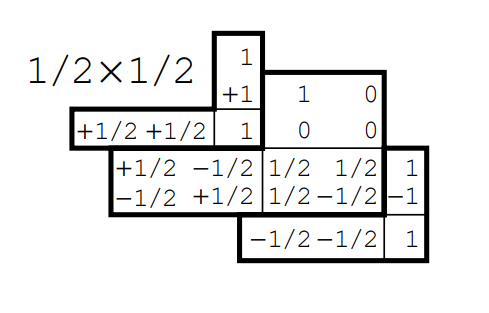
\includegraphics[width=.44\linewidth]{cg_12_12.png}
			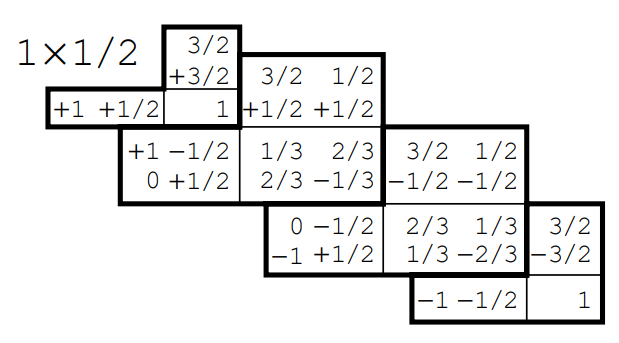
\includegraphics[width=.54\linewidth]{cg_1_12.png}
			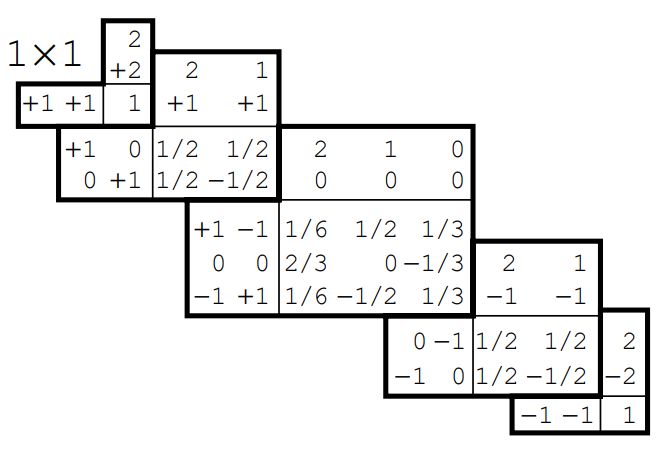
\includegraphics[width=1\linewidth]{cg_1_1.png}
		\end{figure}
\end{itemize}
\end{multicols*}
\end{footnotesize}
\end{document}
